%!TeX encoding=utf8
\documentclass[ngerman]{scrartcl} 

% Passen Sie hier *Author1*, *Author2* und *Grp.-Nr.* an.
\newcommand{\authA}{Alexander Steding}

\newcommand{\grpnr}{4}
\usepackage{array}
\usepackage{longtable}

% Optionen für die Dokumentenklasse scartcl von KOMAscript. 
\KOMAoptions{
	DIV=11,
	BCOR=0mm,
	paper=a4,
	fontsize=12pt,
	parskip=half,
	twoside=false,
	titlepage=false
}
\usepackage{booktabs}

% Papierformat: DIN-A4, mit wenig Rand 
\usepackage[
	a4paper,
	left=20mm,
	right=20mm,
	top=23mm, 
	bottom=18mm,
	includefoot,
	footskip=8mm
	]{geometry}

% Zeilenabstand, andere Werte: onehalfspacing, doublespacing
\usepackage[singlespacing]{setspace} 

% Definition der Kopf- und Fußzeile
\usepackage[headsepline,automark]{scrlayer-scrpage}
\clearscrheadings
\setlength{\headheight}{2.5\baselineskip}
\setlength{\footheight}{1\baselineskip}
\ihead[]{\\ \authA}
\chead[]{ \\  Abschlussbericht}
\ohead[]{ \\  \today }
\ofoot[]{\pagemark}

%---Language and umlauts
\usepackage[utf8]{inputenc}       % UTF-8 Kodierung - ä, ö, ü, ß direkt eingeben
\usepackage[ngerman]{babel}                      % Neue deutsche Rechtschreibung  
\usepackage[expansion=true, protrusion=true]{microtype} % Bessere Silbentrennung

% Formelsatz
\usepackage{amsmath}		% Mathematik-Umgebungen - z.B. align
\usepackage{amsthm}		% Umgebung "theorem"
\usepackage{amsfonts}	% Schriften
\usepackage{amssymb}		% Symbole
\usepackage{upgreek}		% Griechische Sonderzeichen z.B. \upmu
\usepackage{booktabs}
% Einheiten
\usepackage{siunitx}
\sisetup{
	locale = DE,  
	separate-uncertainty,  
	range-units = brackets,  
	list-units = single,  
	per-mode=fraction
}

% Bilder und Tabellen
\usepackage{graphicx}			% Bilder als PDF einbinden
\usepackage{epstopdf}			% Bilder im EPS-Format
\usepackage{caption}				% Unterschriften für Bilder und Tapellen
\usepackage{booktabs}			% Zusätzliche Schönheitslinien für Tabellen
\usepackage{multirow}			% Mehrere Felder in einer Tabelle zusammenfassen
\usepackage[table]{xcolor}		% Für farbig unterlegte Tabellenzeilen
  \definecolor{lightgray}{gray}{0.9}
  \rowcolors{1}{}{lightgray}	% jede zweite Zeile in einer Tabelle leicht grau


% Positionierung von Bildern und Tabellen
\usepackage{float}				% Option 'H', also "hier-egal-wie-das-aussieht"
\usepackage[section]{placeins}	% Platzierung spätestens am Ende eines Kapitels
\renewcommand{\floatpagefraction}{.75}	% standard: .5
\renewcommand{\textfraction}{.1}			% standard: .2
\renewcommand{\topfraction}{.8}			% standard: .7
\renewcommand{\bottomfraction}{.5}		% standard: .3
\setcounter{topnumber}{3}				% standard: 2
\setcounter{bottomnumber}{2}				% standard: 1
\setcounter{totalnumber}{5}				% standard: 3

\usepackage{caption}
\captionsetup[figure]{name=Abb.}
\captionsetup[table]{name=Tab.}

% Hyperlinks
\usepackage{hyperref}
\hypersetup{
	colorlinks=true, 
	breaklinks=true, 
	citecolor=darkgray, 
	linkcolor=darkgray, 
	menucolor=red, 
	urlcolor=cyan,
	bookmarksopen=false, 
	bookmarksopenlevel=0,
	plainpages=false,			% zur korrekten Erstellung der Bookmarks 
	hypertexnames=false			% zur korrekten Erstellung der Bookmarks 
}

\usepackage{pdfpages} 		% Einfügen von Vollseiten-PDFs (z.B. das Deckblatt)
\usepackage{csquotes}		% Zitate
\usepackage{pythonhighlight}
% Literaturverzeichnis
\usepackage[style=alphabetic,sorting=ynt,backend=biber]{biblatex}

% Eine Abkürzung, die Computerbefehle im Fließtext mit einer Mono-Schrift setzt
% (funktioniert leider nicht für Backslash \ . Da hilft dann der Befehl \verb )
\providecommand*{\code}[1]{{\texttt{#1}}}
\usepackage{listings}
\usepackage{xcolor}

\definecolor{codegreen}{rgb}{0,0.6,0}
\definecolor{codegray}{rgb}{0.5,0.5,0.5}
\definecolor{codepurple}{rgb}{0.58,0,0.82}
\definecolor{backcolour}{rgb}{0.95,0.95,0.92}

\lstdefinestyle{mystyle}{
    backgroundcolor=\color{backcolour},   
    commentstyle=\color{codegreen},
    keywordstyle=\color{magenta},
    numberstyle=\tiny\color{codegray},
    stringstyle=\color{codepurple},
    basicstyle=\ttfamily\footnotesize,
    breakatwhitespace=false,         
    breaklines=true,                 
    captionpos=b,                    
    keepspaces=true,                 
    numbers=left,                    
    numbersep=5pt,                  
    showspaces=false,                
    showstringspaces=false,
    showtabs=false,                  
    tabsize=2
}

\lstset{style=mystyle}
\usepackage{hyperref}
\begin{document}
\shorthandoff{"}           % Anführungszeichen nicht als Befehl interpretieren



\begin{titlepage}
\begin{center}
\vspace{3cm}
{\fontsize{40}{49} \selectfont \textbf{Programmierpraktikum}}\\[2cm]
{\fontsize{40}{49} \selectfont \textbf{Der Bericht}}\\[2cm]
\Large{\authA }\\
\Large{10028034 }\\
\large{Gottfried Wilhelm Leibniz Universität\\{\today}}
\end{center}
\end{titlepage}
\stepcounter{page}

\newpage
\tableofcontents
\newpage
\section{Einleitung }
Dieser Bericht stellt als Abschlussbericht die Ergebnisse und Erkenntnisse des Programmierpraktikums Schadstoffausbreitung zusammen. Angefangen mit dem Vergleich zwischen Gauß-Modell und Monte-Carlo-Modell, weiter über die Validierung des Monte-Carlo-Modells und schließlich zur Anwendung des Modells in einer Straßenschlucht. Abschließend werden Gedanken über die dreidimensionale Schadstoffausbreitung  in Stadtgebieten geteilt. Als Programmiersprache wurde über alle Aufgaben hinweg Julia verwendet und als Graphisches Backend PlotlyJS sowie GlMakie.
\section{Aufgabe  1}
Ziel dieser Aufgabe ist es ein Gauß-Modell für eine kontinuierliche Linienquelle zu Programmieren und anschließend die Maximalkonzentration am Erdboden zu bestimmen.

In Aufgabenteil b wird ein Monte-Carlo-Modell für eine kontinuirliche Linienquelle programmiert und mit dem Gauß-Modell aus Aufgabenteil a verglichen.
\subsection{Aufgabenteil a}
In Aufgabenteil a wird zunächst ein Gauß-Modell für die Ausbreitung einer kontinuirliche Linienquelle programmiert mit Vernachlässigung der Prandtlschicht. 
Hier gilt:
\begin{align}
x= 51 \si{m} \\
z= 45 \si{m} \\
q= 540 \frac{\si{kg}}{\si{h}}\\
\tau_{l} =100 \si{s}\\
\sigma_{w}=0.39 \frac{\si{m}}{\si{s}}\\
\end{align}


In Abbildung 1. ist die zu erwartende Konzentrationsverteilung des Gauß-Modells als X-Z-Schnitt visualisiert.
\begin{figure}[H]
	\centering
	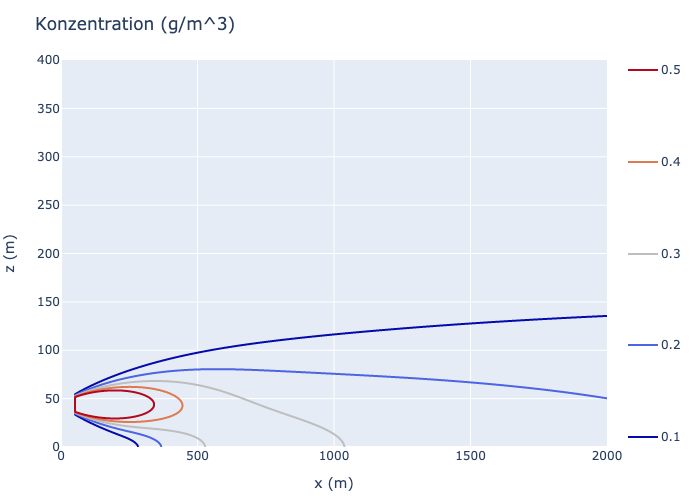
\includegraphics[scale=0.5]{Bilder/1a.png}
	\caption{Konzentrationsverteilung als Contour-Plot. Die Konzentration ist in $\frac{\si{g}}{\si{m^3}}$ dargestellt. }
	\label{fig:my_label}
\end{figure}

Für eine feinere grapische Analyse wurde in Abbildung 2. die Konzentrationsverteilung am Erdboden, also für $z=0\si{m}$, visualisiert.
\begin{figure}[H]
	\centering
	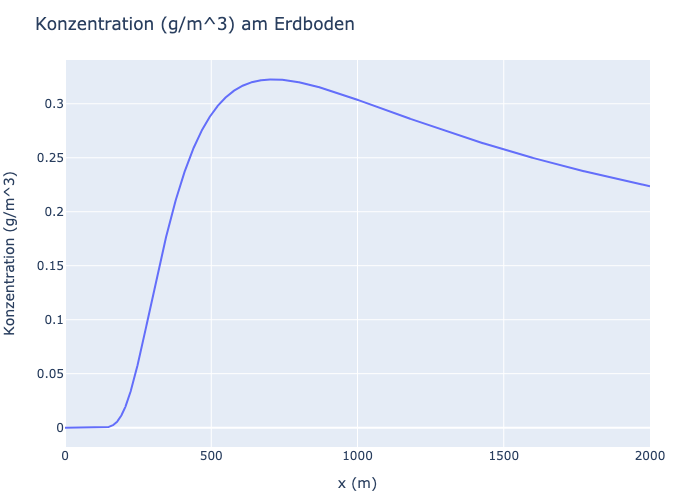
\includegraphics[scale=0.5]{Bilder/1b.png}
	\caption{Konzentrationsverteilung am Erdboden.  Die Konzentration ist in $\frac{\si{g}}{\si{m^3}}$ dargestellt.}
	\label{fig:my_label}
\end{figure}

Die maximale Konzentration wurde final rechnerisch mittels Julia bestimmt als
\begin{equation}
	c[0,711] = 0,32263  \frac{g}{m^3}
\end{equation}
.

\subsection{Aufgabenteil b}
In Aufgabenteil b wird nun das Monte-Carlo-Modell mit einer genährten Gitterauswertung verwendet.
Für den Vergleich zwischen Monte-Carlo-Modell und Gauß-Modell wurden beide Modelle in einem Contour-Plot visualisiert.  Für die optimale Visualisierung wurden verschiedene Partikelanzahlen simuliert.

Zunächst für $N=1000$
\begin{figure}[H]
	\centering
	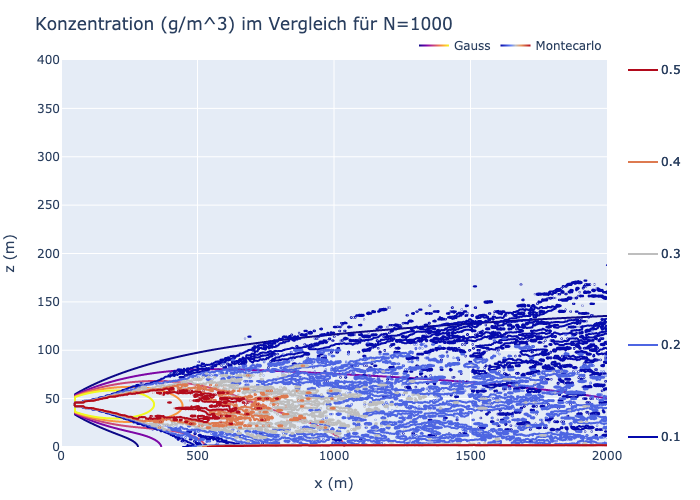
\includegraphics[scale=0.5]{Bilder/1b1k.png}
	\caption{Vergleich für N=1000. Die Konzentration ist in $\frac{\si{g}}{\si{m^3}}$ dargestellt.}
	\label{fig:my_label}
\end{figure}
In Abb. 4 ist leider keine gute Annäherung des Monte-Carlo-Modells an das Gauß-Modell zu erkennen. Die Anzahl der Teilchen hat beim Monte-Carlo-Modell einen hohen Einfluss auf die Güte des Modells. Bei einer geringeren Anzahl wie 

\begin{equation}
	N=1000
\end{equation}
sind extrem große Abweichungen zum Gauß-Modell zu erkennen, obwohl auch hier bereits die Grundstruktur erkennbar ist.
\begin{figure}[H]
	\centering
	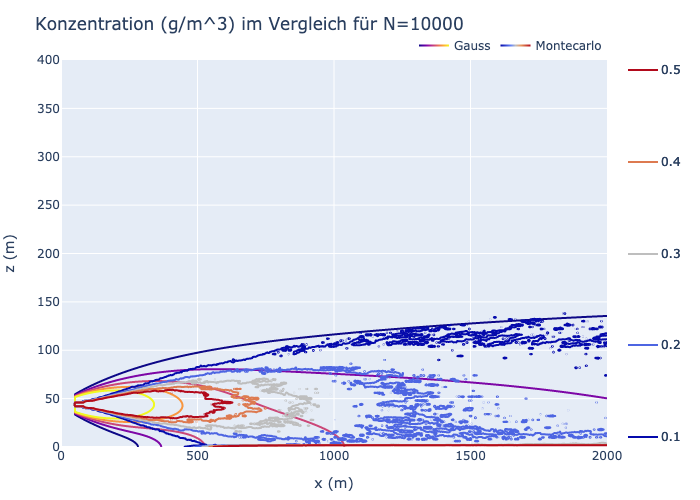
\includegraphics[scale=0.5]{Bilder/1b10k.png}
	\caption{Vergleich für N=10000. Die Konzentration ist in $\frac{\si{g}}{\si{m^3}}$ dargestellt.}
	\label{fig:my_label}
\end{figure}
Bei einer mittleren Anzahl wie 

\begin{equation}
	N=10000
\end{equation}
gleicht sich das Monte-Carlo-Modell bedeutend besser an das Gauß-Modell an.
\begin{figure}[H]
	\centering
	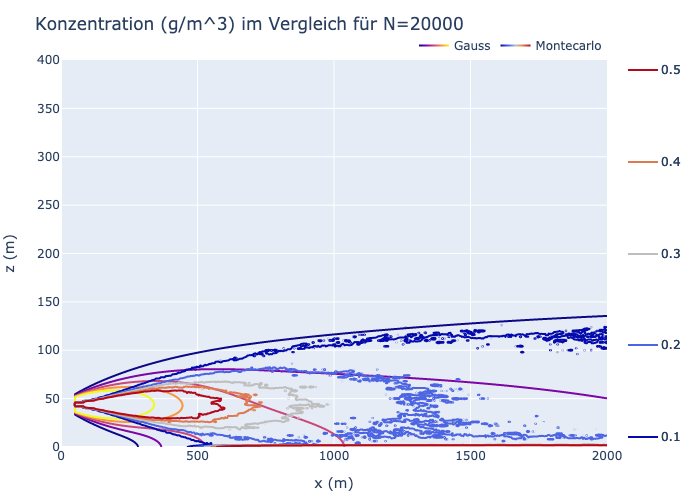
\includegraphics[scale=0.5]{Bilder/1b20k.png}
	\caption{Vergleich für N=20000. Die Konzentration ist in $\frac{\si{g}}{\si{m^3}}$ dargestellt.}
	\label{fig:my_label}
\end{figure}
Bei einer hohen Anzahl wie 

\begin{equation}
	N=20000
\end{equation}
gleicht sich das MC Modell sehr gut an das Gauß-Modell an.
\begin{figure}[H]
	\centering
	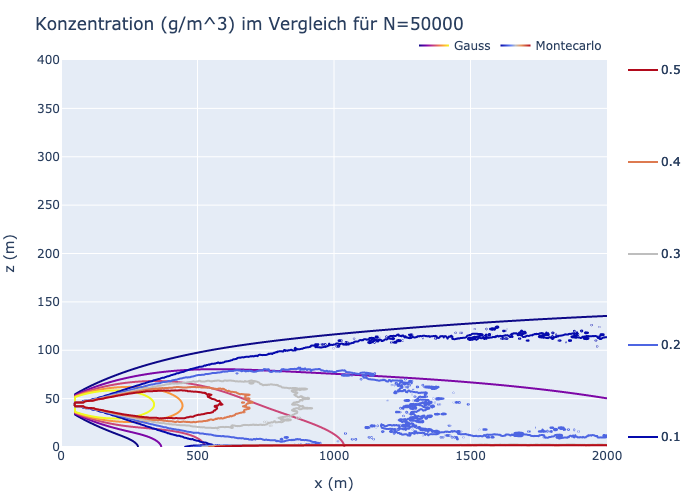
\includegraphics[scale=0.5]{Bilder/1b50k.png}
	\caption{Vergleich für N=50000.  Die Konzentration ist in $\frac{\si{g}}{\si{m^3}}$ dargestellt.}
	\label{fig:my_label}
\end{figure}
Abbildung 6  zeigt das mit meiner Hardware maximal mögliche Ergebnis. Jenseits von dieser Anzahl sind zwar noch leichte Verbesserungen zu erwarten, nichts destotrotz zeigt sich bei 

\begin{equation}
	N=50000
\end{equation}

eine extrem gute Annäherung an das Gauß-Modell. Für eine Ausreichende Statistik reichen aber bereits 
\begin{equation}
	N=20000
\end{equation}.

Die größten Unterschiede zwischen dem Monte-Carlo-Modell und dem Gauß-Modell enstehen bei zunehmender Entfernung von der Quelle, sowie in der Nähe des Quellortes selbst. Auch im Bereich bis 500 m  in X Richtung ist die Konzentration beim Monte-Carlo-Modell niedrieger als beim Gauß-Modell, allen voran aber fehlt hier die Variation der Konzentration, die mit dem Gauß-Modell aufgelöst werden kann. 
\section{Aufgabe 2}
In dieser Aufgabe sollte das Monte-Carlo-Modell mit der Prandtl-Schicht optimiert und die Ergebnisse durch das Prairie-Grass-Experiment validiert werden. Für die Valiedierung wurde ein grafischer Vergleich gewählt. Dazu wurde jeweils die Z-Achse vom Prairie-Grass-Experiment sowie des Monte-Carlo-Modells mit der entsprechenden Konzentration in einem Plot dargestellt. Als Randbedingungen sollen hier gelten:

\begin{align}
	x=0 \si{m} \\
	z= 0.5 \si{m} \\
	z_0 = 0.008 \si{m} \\
	u_{*}=0.35 \frac{\si{m}}{\si{s}}\\
	\kappa =0.38
\end{align}
Im folgenden ist die Konzentrationsverteilung bei $x=100\si{m}$ dargestellt.
\begin{figure}[H]
	\centering
	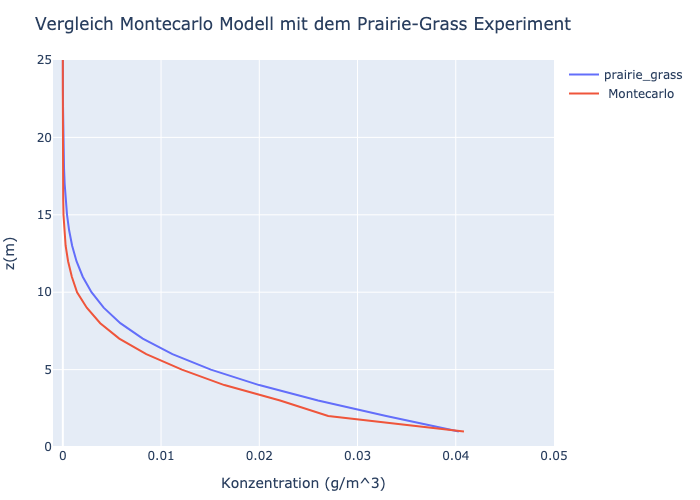
\includegraphics[scale=0.5]{Bilder/2.png}
	\caption{Vergleich Prairie-Grass, Monte-Carlo.  Die Konzentration ist in $\frac{\si{g}}{\si{m^3}}$ dargestellt.}
	\label{fig:my_label}
\end{figure}
Rein Qualitativ betrachtet ist der Verlauf des Monte-Carlo-Modells dem des Prairie-Grass-Experimentes extrem ähnlich. Insbesondere für $z>15 \si{m}$ ist der Unterschied fast verschwindend gering. Die Größte Abweichung bei einer rein qualitativen Betrachtung liegt in Bodennähe bei $z<2 \si{m}$ zu finden.  Trotzdem ist über den gesammten Verlauf der Höhe eine Abweichung von etwa $\Delta c=0.0025 \frac{\si{g}}{\si{m^3}} $
zu beobachten. Zum Erdboden direkt hin konvergieren die beiden Konzentrationen erneut gegeneinader so dass die Unterschiede an dieser Stelle nahezu verschwinden. 

\section{Aufgabe  3}
Ziel dieser Aufgabe ist die Anwendung der bisher verwendeten Monte-Carlo-Methode in einem praxisnahen Beispiels. Dabei wurden die für eine Straßenschlucht mit dem Modell PALM simulierten Windgeschwindigkeiten sowie deren Standartabweichung importiert und ein Contourprofil aus der berechneten Konzentration gebildet. Für die Berechnung von $\tau_l$ wurde der Prandtl-Kolmorov-Ansatz verwendet. Aufgrund der besseren Optimierung wurde für die komplexeren Berechnungen in dieser Aufgabe statt PlotlyJS  GlMakie als Visualiesierungs-Backend verwendet.
Im ersten Szenario wurde ein Schadstoffquelle im Straßenverkehr mit Quellort 
\begin{align}
	x=60.5 \si{m} \\
	z= 0.5 \si{m} 
\end{align}
simuliert.
\begin{figure}[H]
	\centering
	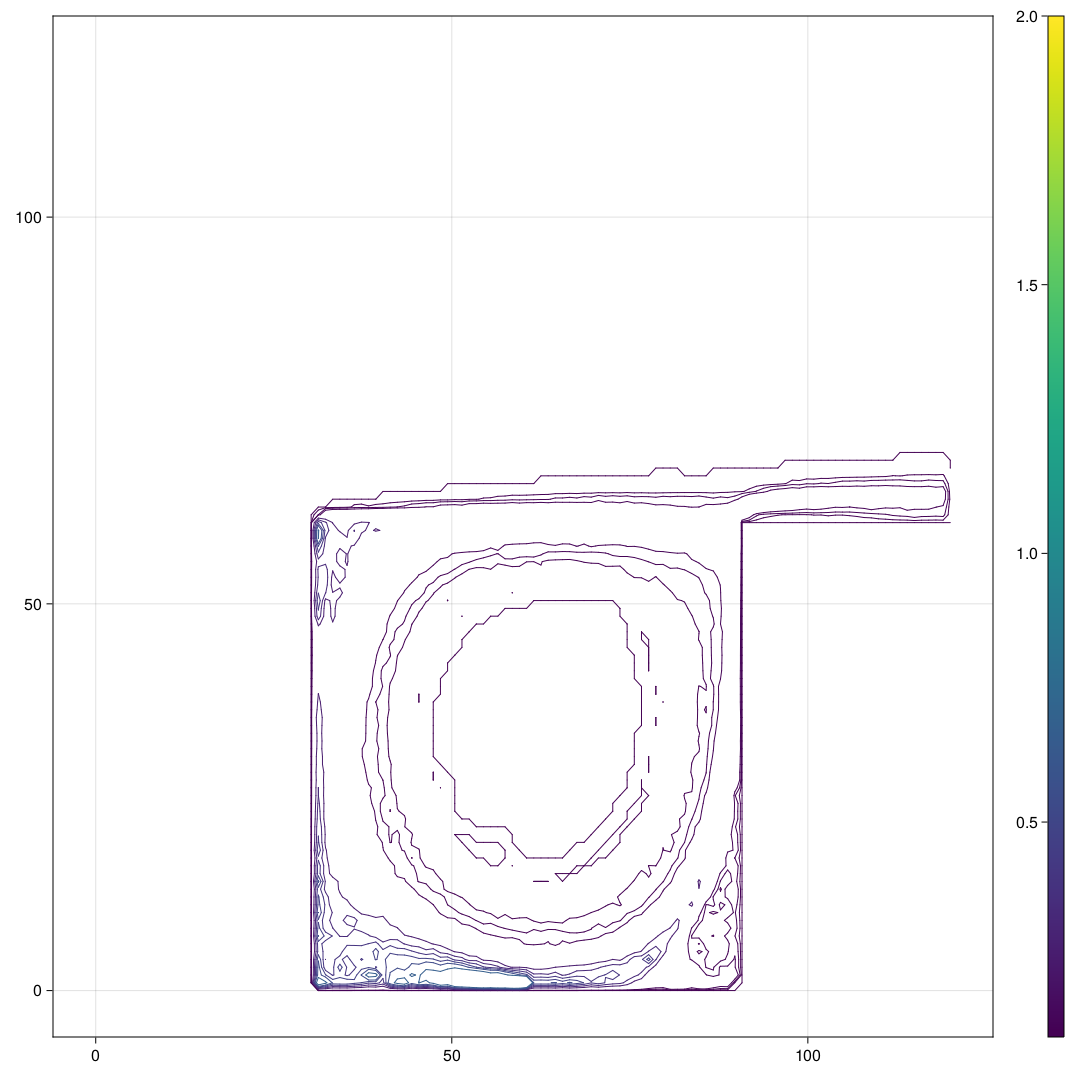
\includegraphics[scale=0.25]{Bilder/3_single_x = 60.5.png}
	\caption{Konzentrationsverteilung am Erdboden. Die Konzentration ist in $\frac{\si{kg}}{\si{s}}$ dargestellt. N=1000, $\lambda =5$}
	\label{fig:my_label}
\end{figure}
In der Straßenschlucht bildet sich durch den Wind über der Schlucht ein Wirbel aus. In diesem sinkt die Konzentration mit abnehmendem Abstand zum Zentrum, sowie tendenziel mit der Höhe. Besonders am Boden der Lee-Seite der Straßenschlucht kommt es zu einer extrem starken Ansammlung der Schadstoffe. Teilweise sind dort um den Faktor 500 höhere Konzentrationen simuliert worden als im Zentrum des Wirbels. Dies kann zu je nach Schadtstoff zu negativen gesundheitlichen Folgen für Fußgänger*innen, Radfahrer*innen, Anwohner*innen, welche sich in der Nähe aufhalten führen.


Im zweiten Szenario wurde als  Schadstoffquelle ein Hausbrand mit Quellort
\begin{align}
	x=15.5 \si{m} \\
	z= 65.5 \si{m} 
\end{align}
simuliert.
\begin{figure}[H]
	\centering
	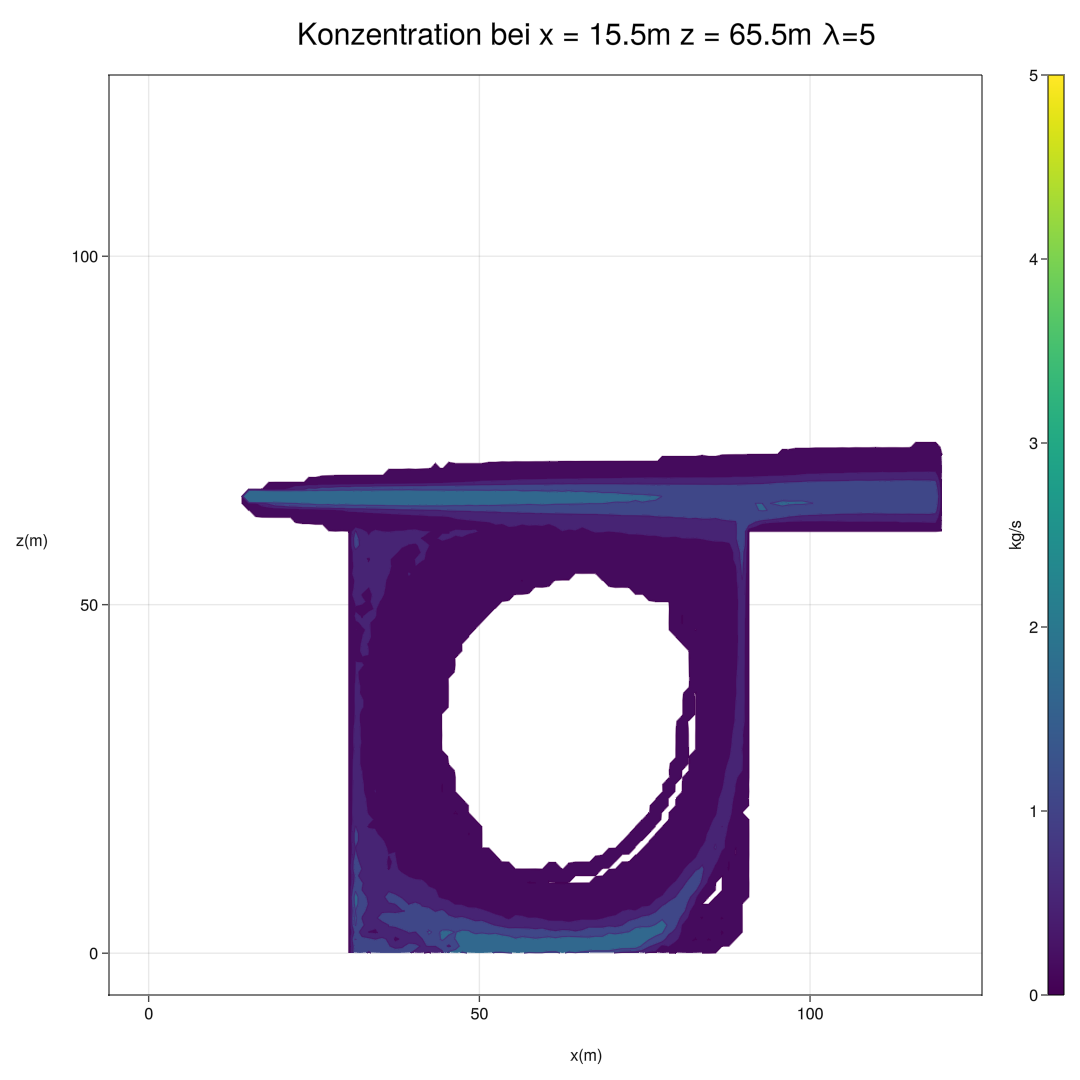
\includegraphics[scale=0.3]{Bilder/3_single_x = 15.5.png}
	\caption{Konzentrationsverteilung am Erdboden. Die Konzentration ist in $\frac{\si{kg}}{\si{s}}$ dargestellt.N=1000, $\lambda =5$}
	\label{fig:my_label}
\end{figure}
Abseits der offensichtlichen Änderung durch den neuen Quellort über den Häusern, zeigt sich ein nahezu ähnliches Bild wie im ersten Szenario. Erneut befindet sich der Ort der größten Konzentration an Schadstoffen in Bodennähe. Ein signifikanter Unterschied ist jedoch die quantitative  Konzentrationshöhe am Erdboden. Diese liegt mit $c= 2,5 \frac{\si{kg}}{\si{s}}$ nur noch halb so hoch wie im vorherigen Fall. Die allgemein geringere Konzentration lässt sich auf die Quellposition über der Häuserschlucht zurückführen, wodruch nur noch ein Teil der Partikel in den Wirbel gelangen kann.
\subsection{Einfluss der Teilchenanzahl}
Desweiteren soll nun der Einfluss der Teilchenanzahl analysiert werden. Dazu wurde für jedes Szenario ein Plot, welcher vier Contourplots für unterschiedliche Partikelanzahlen im direkten Vergleich visualisiert gewählt.
\begin{figure}[H]
	\centering
	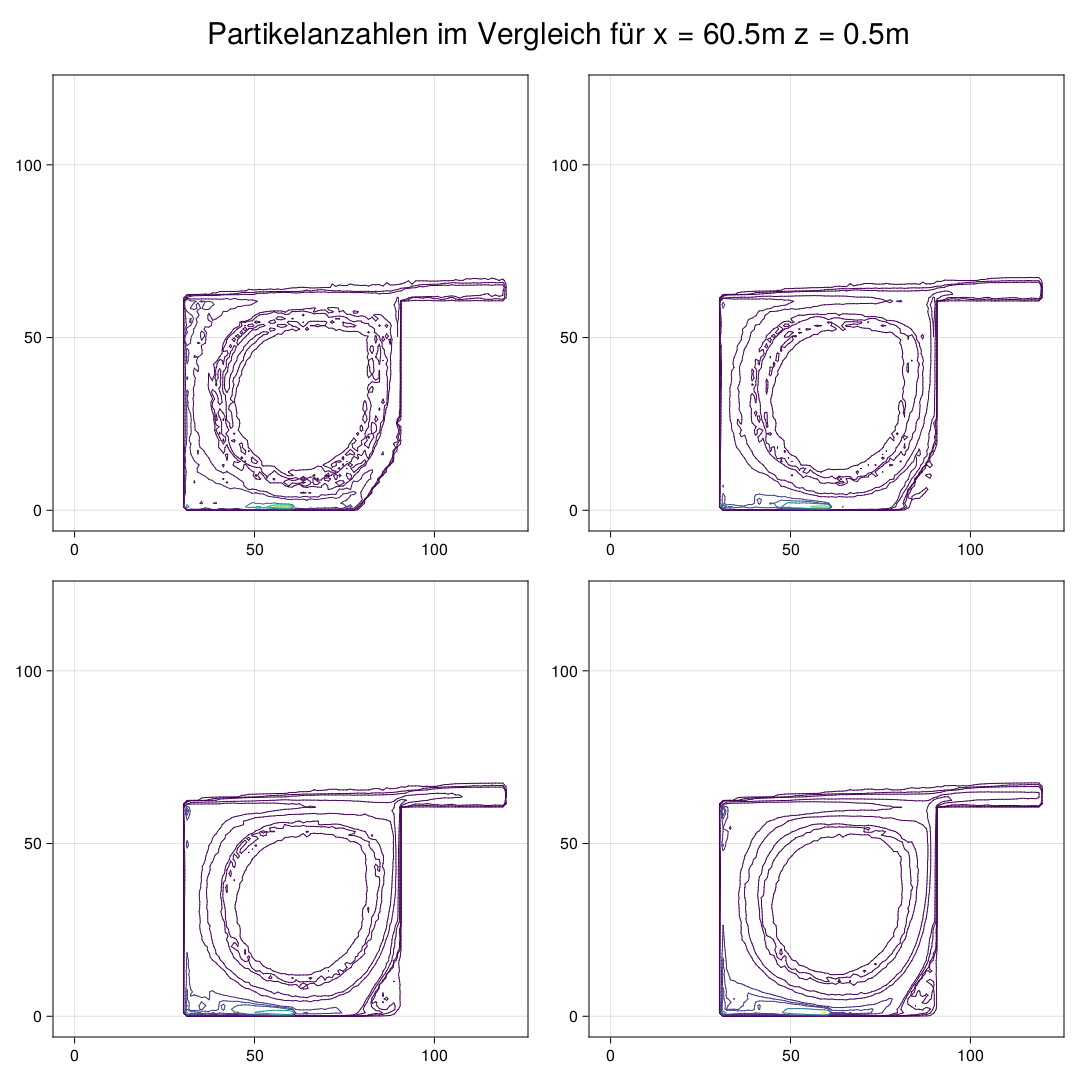
\includegraphics[scale=0.25]{Bilder/3_vergleich_x = 60.5.png}
	\caption{ Verschiedene Konzentrationsverteilung im Vergleich. $N \in[10^2,10^3,5 *10^3,10^4]$ v.L.n.R.  $\lambda =5$}
	\label{fig:my_label}
\end{figure}
Für die Situation a) bringt eine Erhöhung der Teilchenzhahl von $ N=100$ dargestellt in Abblidung 10 linksoben auf  $ N=1000$ einen enormen Sprung in der Qualität der Konzentration. Dadurch können so zum Beispiel auch die feineren Wirbelstrukturen im Zentrum der Häuserschlucht erfasst werden. Eine weitere Erhöhung auf $N=5000$ ermnöglicht  noch eine gering höhere Auflösung; $N=10000$ führen trotz höherer Rechenzeit nur zu einer marginalen Verbesserung. Aus ökonomischen Gesichtspunkten ist eine Teilchenanzuahl zwischen 1000 und 5000 optimal.

\begin{figure}[H]
	\centering
	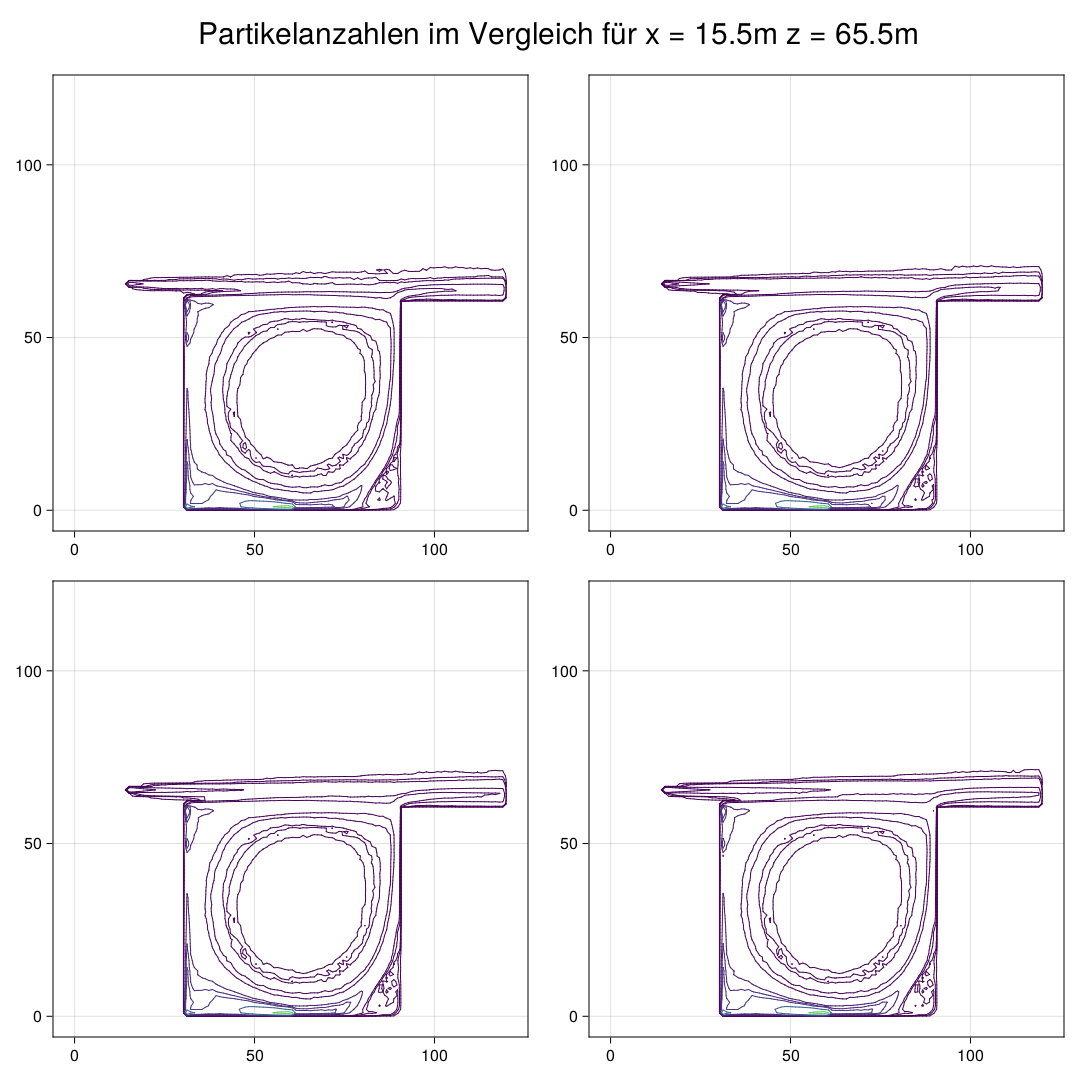
\includegraphics[scale=0.25]{Bilder/3_vergleich_x = 15.5.png}
	\caption{ Verschiedene Konzentrationsverteilung im Vergleich. $N \in[10^2,10^3,5 *10^3,10^4]$v.L.n.R, $\lambda =5$}
	\label{fig:my_label}
\end{figure}
Für die in Aufgabenteil b) geschilderte Situation zeichnet sich ein leicht anderer Verlauf ab. Zwischen $N=100$ und $N=1000$ ist auch hier der Qualitätssprung gut zu erkennen. Im Unterschied zur vorausgegangenen Simulation führt eine Steigerung der Partikelanzahl jenseits von $N=1000$ weiterhin zu einer deutlichen Verbesserung. Da aufgrund der Quellposition bei diesem Szenario weniger Partikel in den Wirbel gelangen, muss für eine repräsentative Darstellung eine höhere Teilchenzahl als bei Situtation a) verwendet werden.


\subsection{Einfluss von $\lambda$ }
Auch der Einfluss von $\lambda$ aus dem Prandt-Kolmogorov-Ansatz soll nun analog betrachtet werden. 
\begin{figure}[H]
	\centering
	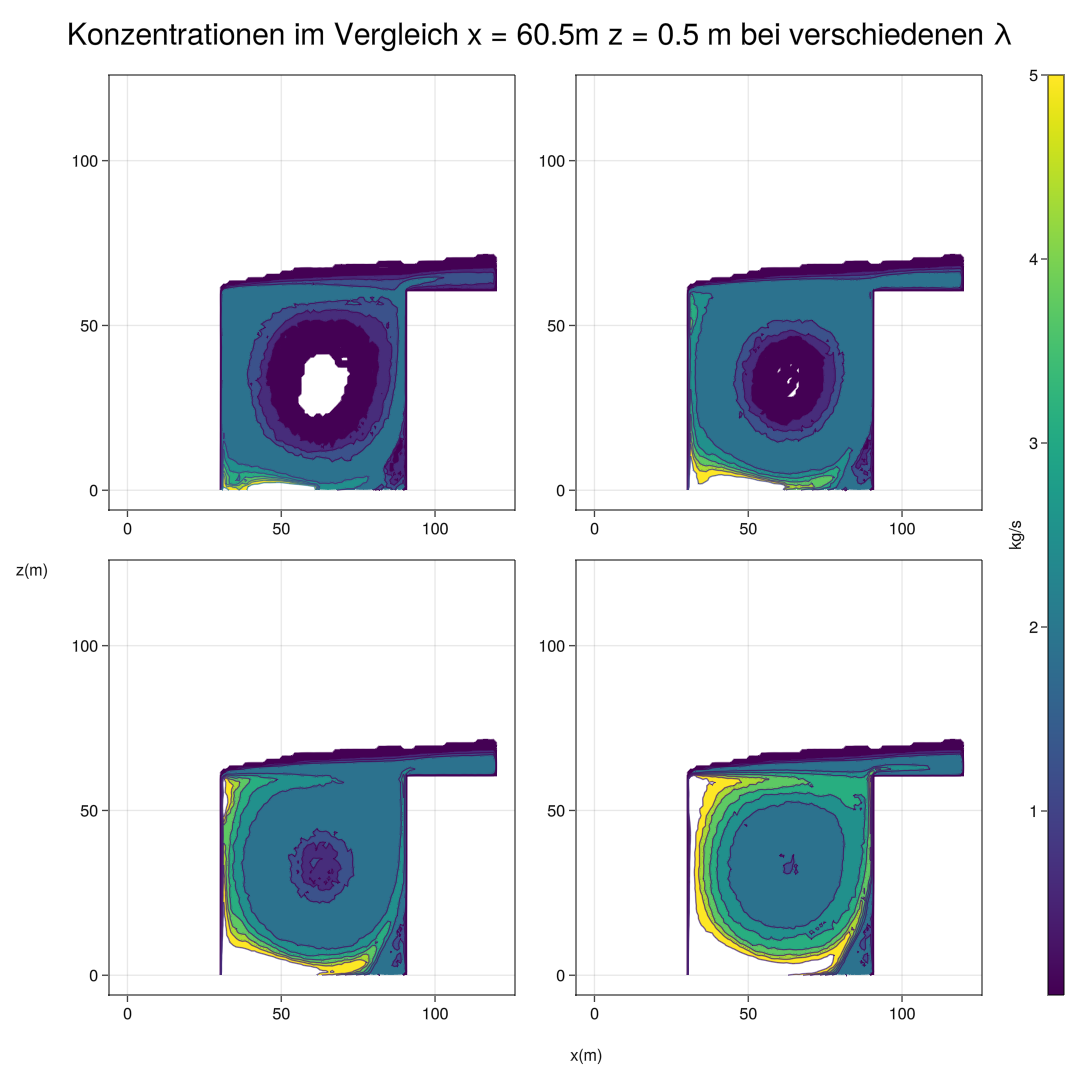
\includegraphics[scale=0.25]{Bilder/3_lambda_x = 60.5.png}
	\caption{Verschiedene $\lambda$ im Vergleich. $\lambda \in[10,5 ,2,1]$ v.L.n.R, N=1000}
	\label{fig:my_label}
\end{figure}

Da es sich bei $\lambda$ um eiine Komponente des Mischungsweg handelt, führt eine Vergrößerung dieses zu einer Vergößerung des Wirbels, et vicae versa. Bei kleinem Mischungsweg kommt es daher in einem deutlich erhöhtem Bereich zu einer Ansammlung gefährlicher Konzentrationen, bei einem großen Mischungsweg zu einer örtlich beschränkteren Ausbreitung.
\subsection{Einfluss von $\sigma$ }
Als letztes soll nun der Einfluss von $\sigma_u$ und $\sigma_w$analog betrachtet werden. Es wurden jeweils beide Standartabweichungen simultan verändert.
\begin{figure}[H]
	\centering
	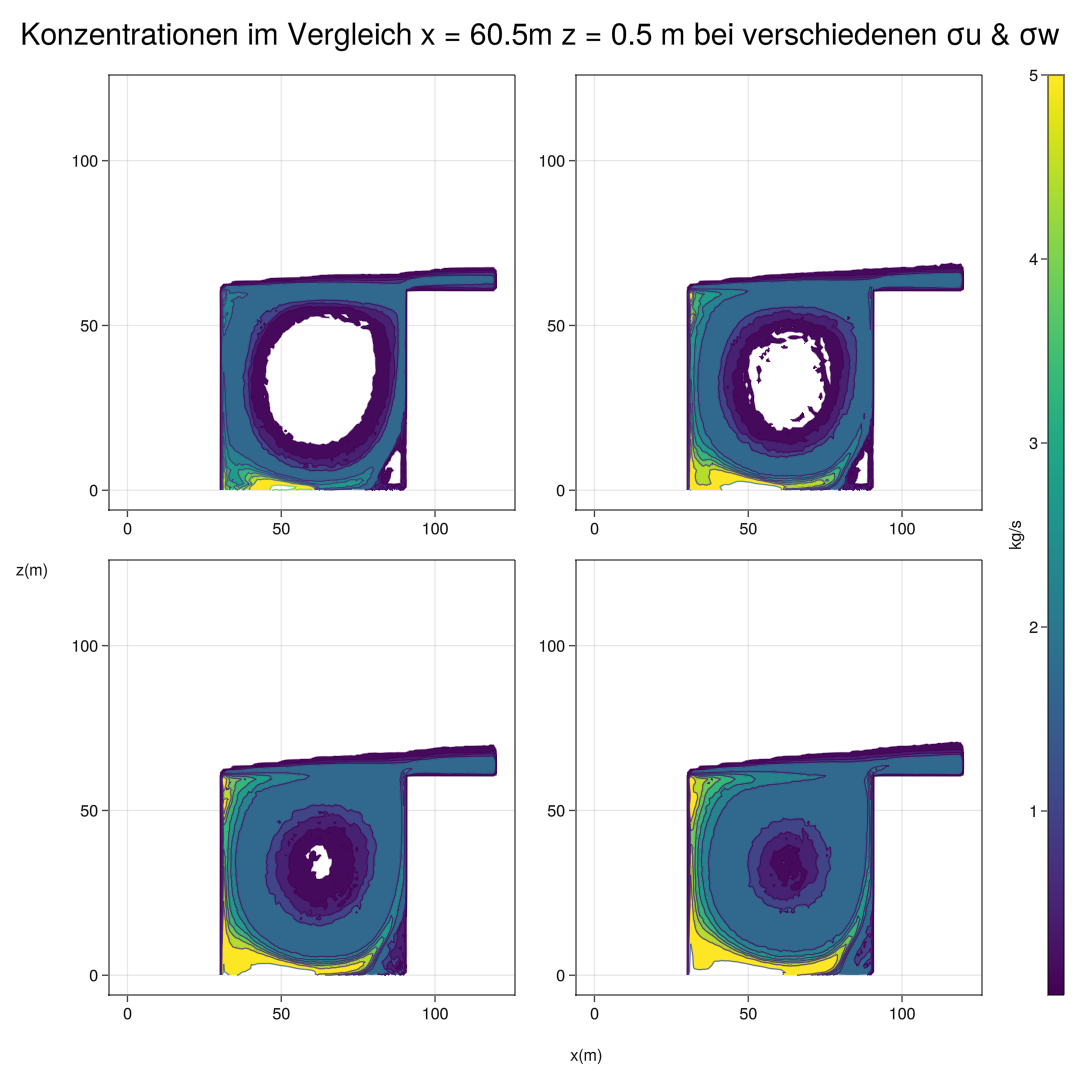
\includegraphics[scale=0.25]{Bilder/3_sigma_x = 60.5.png}
	\caption{Verschiedene $\sigma$ im Vergleich. $\sigma \in[1,2 ,5,10]$ v.L.n.R N=1000, $\lambda =5$}
	\label{fig:my_label}
\end{figure}
Eine Veränderung der Standartabweichung hat in diesem Simulations-Modell direkten Einfluss auf den turbolenten Anteil der Geschwindigkeitskomponente. Eine Zunahme der Standartabweichung führt folglich zu einem stärker ausgeprägtem Wirbel, eine Reduzierung zu einem schwächerem. Analog dazu verhällt sich aufgrund der varierenden Diffusionsstärke jeweils die Konzentration. Wodurch bei einem hohen $\sigma$ eine erhöhte Konzentration auch an den Häuserwänden zu beobachten ist.
\section{Aufgabe  4}
Bei einer Ausbreitung in einem dreidmensionalem Stadtgebiet müssten neben der zusätlichen räumlichen Ausbreitungskoordinate, auch die neue Gitterdimension, sowie die Windkomponenten angepasst und erweitert werden. Auch muss überlegt werden ob statt dem Mischungsweg  der turbolente Diffusionskoeffitient als multidimensionale Größe verwendet werden kann. Dieser könnte möglicherweise aus dem Strömungsmodell stammen.
\newpage
\section{Quellcode}
\subsection{Aufgabe 2}
\lstinputlisting[language=Python]{Aufgabe2.jl}
\subsection{Aufgabe 3}
\lstinputlisting[language=Python]{Aufgabe3.jl}
\end{document}
